% Exam Template for UMTYMP and Math Department courses
%
% Using Philip Hirschhorn's exam.cls: http://www-math.mit.edu/~psh/#ExamCls
%
% run pdflatex on a finished exam at least three times to do the grading table on front page.
%
%%%%%%%%%%%%%%%%%%%%%%%%%%%%%%%%%%%%%%%%%%%%%%%%%%%%%%%%%%%%%%%%%%%%%%%%%%%%%%%%%%%%%%%%%%%%%%

% These lines can probably stay unchanged, although you can remove the last
% two packages if you're not making pictures with tikz.
\documentclass[11pt]{exam}
\RequirePackage{amssymb, amsfonts, amsmath, latexsym, verbatim, xspace, setspace}
\RequirePackage{tikz, pgflibraryplotmarks}

% By default LaTeX uses large margins.  This doesn't work well on exams; problems
% end up in the "middle" of the page, reducing the amount of space for students
% to work on them.
\usepackage[margin=1in]{geometry}

\usetikzlibrary{calc}
\usepackage{graphicx}

% Here's where you edit the Class, Exam, Date, etc.
\newcommand{\class}{Introduction a l'informatique}
\newcommand{\term}{X1I0010, groupe 140}
\newcommand{\examnum}{CC 1}
\newcommand{\examdate}{25/10/2016}
\newcommand{\timelimit}{60 Minutes}

\usepackage{fancyvrb}
\fvset{frame=single,framesep=1mm,fontfamily=courier,fontsize=\normalsize,numbers=left,framerule=.3mm,numbersep=1mm,commandchars=\\\{\}}
\definecolor{dgreen}{rgb}{0.0, 0.5, 0.0}
\definecolor{ballblue}{rgb}{0.13, 0.67, 0.8}

\usepackage[absolute,overlay]{textpos}
\usepackage{caption}

% For an exam, single spacing is most appropriate
\singlespacing
% \onehalfspacing
% \doublespacing

% For an exam, we generally want to turn off paragraph indentation
\parindent 0ex

\begin{document} 

\begin{tikzpicture}[overlay, remember picture]
\node[anchor=north west, %anchor is upper left corner of the graphic
      xshift=2.5cm, %shifting around
      yshift=-0.8cm] 
     at (current page.north west) %left upper corner of the page
     {
\includegraphics[width=16.4cm]{UN_logo.png}}; 
\end{tikzpicture}

% These commands set up the running header on the top of the exam pages
\pagestyle{head}
\firstpageheader{}{}{}
\runningheader{\class}{\examnum\ - Page \thepage\ of \numpages}{\examdate}
\runningheadrule

\begin{flushright}
\begin{tabular}{p{2.8in} r l}
\textbf{\class} && \\%\makebox[2in]{\hrulefill}\\
\textbf{\term} &&\\
\textbf{\examnum} &&\\
\textbf{\examdate} &&\\
\textbf{Dur\'{e}e: \timelimit} & \textbf{Nom, Pr\'enom:} & \makebox[2in]{\hrulefill}
\end{tabular}\\
\end{flushright}
\rule[1ex]{\textwidth}{.1pt}

\noindent\fbox{%
\parbox{0.98\textwidth}{%
\textbf{Pr\'eambule} : Aucun document autoris\'e. Calculatrices et t\'el\'ephones portables interdits. Les exercices ne sont pas class\'es par difficult\'e croissante. Nombre de pages : \numpages.
}%
}
\vspace{12pt}

%\begin{minipage}[t]{3.7in}
%\vspace{0pt}
%\begin{itemize}
%
%\item \textbf{If you use a ``fundamental theorem'' you must indicate this} and explain
%why the theorem may be applied.
%
%\item \textbf{Organize your work}, in a reasonably neat and coherent way, in
%the space provided. Work scattered all over the page without a clear ordering will 
%receive very little credit.  
%
%\item \textbf{Mysterious or unsupported answers will not receive full
%credit}.  A correct answer, unsupported by calculations, explanation,
%or algebraic work will receive no credit; an incorrect answer supported
%by substantially correct calculations and explanations might still receive
%partial credit.
%
%
%\item If you need more space, use the back of the pages; clearly indicate when you have done this.
%\end{itemize}
%
%Do not write in the table to the right.
%\end{minipage}
%\hfill
%\begin{minipage}[t]{2.3in}
%\vspace{0pt}
%%\cellwidth{3em}
%\gradetablestretch{2}
%\vqword{Problem}
%\addpoints % required here by exam.cls, even though questions haven't started yet.	
%\gradetable[v]%[pages]  % Use [pages] to have grading table by page instead of question
%
%\end{minipage}
%	\newpage % End of cover page

%%%%%%%%%%%%%%%%%%%%%%%%%%%%%%%%%%%%%%%%%%%%%%%%%%%%%%%%%%%%%%%%%%%%%%%%%%%%%%%%%%%%%
%
% See http://www-math.mit.edu/~psh/#ExamCls for full documentation, but the questions
% below give an idea of how to write questions [with parts] and have the points
% tracked automatically on the cover page.
%
%
%%%%%%%%%%%%%%%%%%%%%%%%%%%%%%%%%%%%%%%%%%%%%%%%%%%%%%%%%%%%%%%%%%%%%%%%%%%%%%%%%%%%%

\begin{questions}

% Basic question
%\addpoints
\question \'Ecrire un algorithme demandant \`a l'utilisateur de saisir un nombre. L'algorithme doit ensuite afficher un message indiquant si ce nombre est \textbf{premier}. 

Un nombre \textbf{premier} est un entier naturel qui admet exactement deux diviseurs distincts entiers et positifs (qui sont alors 1 et lui-m\^eme). Ainsi, $1$ n'est pas premier car il n'a qu'un seul diviseur entier positif; $0$ non plus car il est divisible par tous les entiers positifs.

% Question with parts
%\newpage
%\addpoints
\question On suppose disposer de la fonction :

\begin{Verbatim}
\textcolor{blue}{\bf fonction} \textcolor{ballblue}{\bf etoile}(nomb : \textcolor{dgreen}{entier}) : \textcolor{dgreen}{chaine}
{\bf Variables}
	etoiles : \textcolor{dgreen}{chaine}
	i : \textcolor{dgreen}{entier}
{\bf Debut}
	etoiles <- ""
	\textcolor{blue}{\bf pour} i \textcolor{blue}{\bf allant de} 1 \textcolor{blue}{\bf a} nomb \textcolor{blue}{\bf faire} 
		etoiles <- etoiles + "*"; 
	\textcolor{blue}{\bf fin pour}
	\textcolor{blue}{\bf retourner} (etoiles) 
{\bf Fin}
\end{Verbatim}

En utilisant la fonction \textcolor{ballblue}{\bf etoile}, \'ecrire un algorithme affichant le texte suivant :

\begin{figure}[h!]
\centering
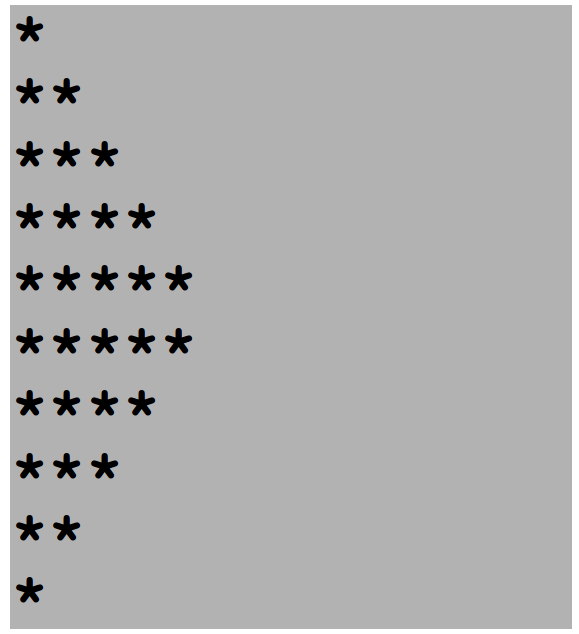
\includegraphics[height=5cm]{out1.png}
\captionsetup{labelformat=empty}
%\caption{Une figure.}
\end{figure}

%\begin{parts}
%\part[5] Find $f'(x)$ using the limit definition of derivative.
%\vfill
%\part[5] Find the line tangent to the graph of $y=f(x)$ at the point where $x=2$.
%\vfill
%\end{parts}

% If you want the total number of points for a question displayed at the top,
% as well as the number of points for each part, then you must turn off the point-counter
% or they will be double counted.
\newpage
%\addpoints
\question La \textit{\bf suite de Fibonacci} est une suite d'entiers dans laquelle chaque terme est la somme des deux termes qui le pr\'ec\`edent. Elle commence g\'en\'eralement par les termes $0$ et $1$ et ses premiers termes sont : $0, 1, 1, 2, 3, 5, 8, 13, 21,\dots$ etc.

Formellement, la \textit{\bf suite de Fibonacci} est d\'efinie comme suit :

\begin{align*}
f_0 &= 0\\
f_1 &= 1\\
f_n &= f_{n-1} + f_{n-2}
\end{align*}

\'Ecrire une fonction \textcolor{ballblue}{\bf fibo} qui prend en entr\'ee un entier et retourne le N-i\`eme terme de la \textit{\bf suite de Fibonacci}.
%\noaddpoints % If you remove this line, the grading table will show 20 points for this problem.




%\begin{parts}
%\part[5] Find $f'(x)$ using the limit definition of derivative.
%\vspace{4.5in}
%\part[5] Find the line tangent to the graph of $y=f(x)$ at the point where $x=2$.
%\end{parts}



\end{questions}
\end{document}